\documentclass[11pt]{article}
\usepackage{hyperref}
\usepackage[letterpaper, margin=1.2in]{geometry}
% \geometry{letterpaper}
\usepackage{graphicx}
\usepackage{amssymb}
\usepackage{amsmath}
\usepackage{amsthm}
\usepackage{epstopdf}
\usepackage{bbm}
\usepackage{xcolor}
\usepackage{color}
\usepackage{xspace}
\usepackage{longtable}
\usepackage{verbatim}
\usepackage{authblk}
\usepackage{textcomp}
\RequirePackage{palatino}

% packages that I imported
\usepackage{etoolbox}
\usepackage{xr}
\usepackage{caption}
\usepackage{subcaption}
\makeatletter
\newcommand*{\addFileDependency}[1]{% argument=file name and extension
  \typeout{(#1)}
  \@addtofilelist{#1}
  \IfFileExists{#1}{}{\typeout{No file #1.}}
}
\makeatother
\newcommand*{\myexternaldocument}[1]{%
    \externaldocument{#1}%
    \addFileDependency{#1.tex}%
    \addFileDependency{#1.aux}%
}
\externaldocument{main}

\usepackage{algorithm}
\usepackage{algpseudocode}
\usepackage{multicol}
\usepackage{mathtools}
\usepackage{minibox}
\usepackage [autostyle, english = american]{csquotes}
\MakeOuterQuote{"}
\usepackage{caption}
\captionsetup{format=plain, font=small, labelfont=bf}
\usepackage{capt-of}


\newcounter{equationset}
\newcommand{\equationset}[1]{% \equationset{<caption>}
  \refstepcounter{equationset}% Step counter
  \noindent\minibox[c]{Derivation~\theequationset: #1}}% Print caption

\newcommand{\centered}[1]{\begin{tabular}{l} #1 \end{tabular}}

% \usepackage{etoolbox} % for the trick

% % setup algorithmic to use straight quotes
% \AtBeginEnvironment{algorithmic}{\useupquotes}

% % define the command that activates the quotes and redefines them
% \newcommand{\useupquotes}{%
%   \begingroup\lccode`\~=`\'\lowercase{\endgroup\let~}\algoupquote
%   \begingroup\lccode`\~=`\"\lowercase{\endgroup\let~}\algoupquotes
%   \catcode`\'=\active\catcode`\"=\active
% }
% % Customize here (\mbox is necessary because of math mode;
% % if needed in subscripts, use \text instead)
% \newcommand{\algoupquote}{\mbox{\textquotesingle}}
% \newcommand{\algoupquotes}{\mbox{\char`\"}}

\newtheorem{property}{Property}

\newif\ifrevision
\revisionfalse
% \revisionfalse

\newif\ifrevtwo
% \revtwotrue
\revtwofalse

\newif\ifpreprint
% \preprinttrue
\preprintfalse

\newif\ifshowsupp
% \showsupptrue
\showsuppfalse

\ifrevision
\newcommand{\ad}[1]{\textcolor{red}{#1}}
\else
\newcommand{\ad}[1]{\textcolor{black}{#1}}
\fi

\ifrevtwo
\newcommand{\adtwo}[1]{\textcolor{red}{#1}}
\else
\newcommand{\adtwo}[1]{\textcolor{black}{#1}}
\fi

\ifpreprint
% \usepackage[backend=biber,style=numeric,maxbibnames=10,minbibnames=10,sorting=none]{biblatex}
\usepackage[backend=biber,style=nature,maxbibnames=10,minbibnames=10,sorting=none]{biblatex}
\addbibresource{main.bib}
\else
%\usepackage{cite}
\usepackage[round, sort, numbers]{natbib}
\newcommand{\autocite}[1]{\cite{#1}}
\fi

\newcommand{\BTL}[1]{\textcolor{blue}{[\textbf{BTL: #1}]}}
\newcommand{\KC}[1]{\textcolor{red}{[\textbf{KC: #1}]}}
\newcommand{\PC}[1]{\textcolor{orange}{[\textbf{PC: #1}]}}
% \renewcommand{\thefigure}{S\arabic{figure}}
\renewcommand{\figurename}{Figure S\hspace{-3pt}}
\renewcommand{\tablename}{Table S\hspace{-3pt}}

\begin{document}

\pagenumbering{gobble}


%\section*{Figure S1: }
\label{appendix:compression_metrics}

\section{Supplementary Methods}

\subsection{Quantification of public interval collections}

\subsection{Alternative \texttt{subB} sampling strategies and implementation details}

\section{Supplementary Results}

\subsection{Comparison of mixed-stride, hash-threshold, and single-hash subsampling}

\subsection{Interval accuracy at the default precision}

\begin{figure}[htbp]
    \centering
    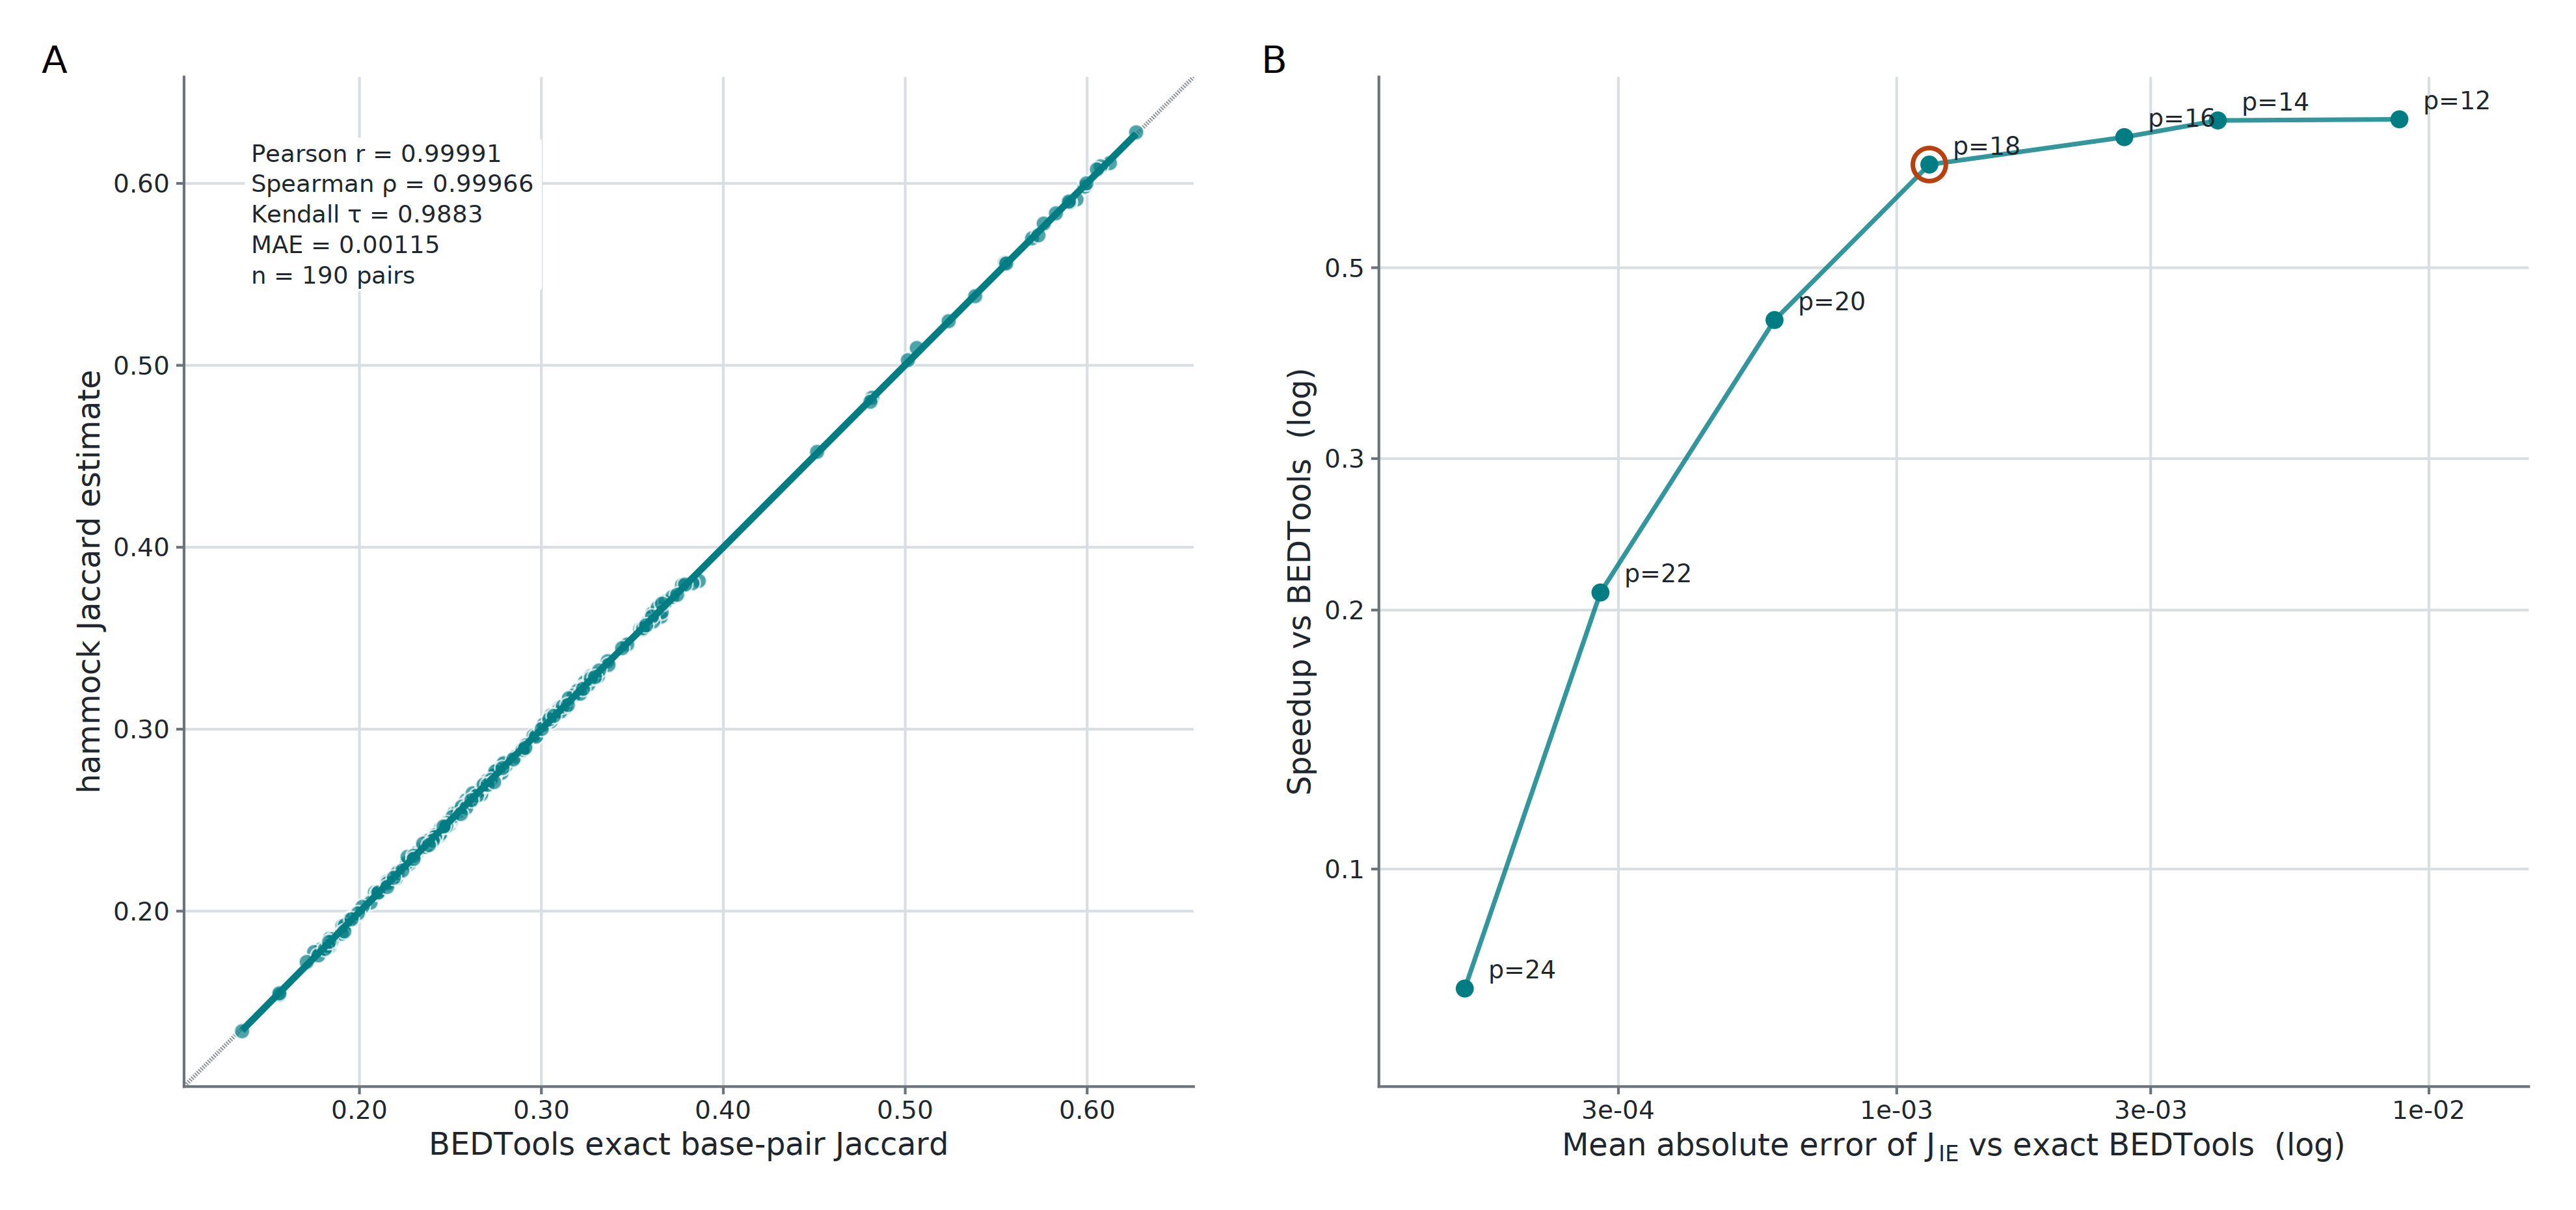
\includegraphics[width=\linewidth]{figures/interval_accuracy_p18.png}
    \caption{\textbf{Inclusion--exclusion estimates closely reproduce exact interval Jaccard at the default HyperLogLog precision.} (A) Pairwise comparisons on 20 Maurano et al. fetal-tissue DNase hypersensitivity BED files yielded 190 unique off-diagonal pairs after self-comparisons and reciprocal duplicates were excluded. At the \program{hammock} command-line default, $p=18$, \texttt{jaccard\_similarity\_ie} closely tracked exact BEDTools base-pair Jaccard (MAE $=0.00115$, Pearson $r=0.99991$, and Kendall $\tau=0.9883$). (B) The precision--runtime analysis from Figure~\ref{fig:interval_accuracy} is repeated for context. Across $p=12$--24, accuracy is the MAE over the same 190 unique pairs and wall time is the median of three complete all-pairs runs using 16 threads and \texttt{subB}=1.0; vertical ranges show the observed replicate range. The circled $p=18$ point marks the command-line default.}
    \label{fig:interval_accuracy_p18}
\end{figure}

\subsection{Register-equality and inclusion--exclusion estimate different quantities}

Figure~\ref{fig:interval_accuracy} evaluates only the numerical accuracy of \texttt{jaccard\_similarity\_ie} relative to exact BEDTools Jaccard. Hammock also emits \texttt{reg\_eq\_similarity}, a register-equality statistic defined as the fraction of active HyperLogLog registers whose values agree. This statistic is not set Jaccard: registers can tie by chance, producing a positive chance-agreement floor whose magnitude depends on sketch load and on the cardinality ratio $|A|/|B|$.

In separate analyses on the same 20-file Maurano et al. fetal-tissue subset, register-equality preserved the broad ordering of pairwise similarities but did not reproduce exact Jaccard magnitudes. At $p=21$, register-equality had MAE $=0.1378$, Pearson $r=0.99720$, and Kendall $\tau=0.9511$ relative to BEDTools Jaccard, whereas inclusion--exclusion had MAE $=4.3\times10^{-4}$, Pearson $r=0.99999$, and Kendall $\tau=0.9947$. The register-equality offset was approximately $0.14$ and remained largely unchanged across $p=18$, $p=21$, and $p=23$, consistent with an estimator-specific chance-agreement floor rather than ordinary sketch sampling error. By contrast, inclusion--exclusion error decreased with precision.

The ordering differences under register-equality were small but systematic. Of the 17,955 possible comparisons between pairs of the 190 similarity observations, register-equality and BEDTools disagreed on the relative ordering of 439 (2.45\%), corresponding to Kendall $\tau=0.951$; all involved BEDTools Jaccard differences below 0.025. The same residual pattern recurred across independently generated sketch sets at $p=18$ and $p=21$ ($r=0.994$), consistent with the chance floor changing with the relative cardinalities of the compared interval sets. Under inclusion--exclusion at $p=21$, the two methods disagreed on 48 such orderings (0.27\%). These analyses explain why the main-text Figure~\ref{fig:interval_accuracy} focuses on inclusion--exclusion when the goal is to recapitulate exact Jaccard values.

\begin{figure}[htbp]
    \centering
    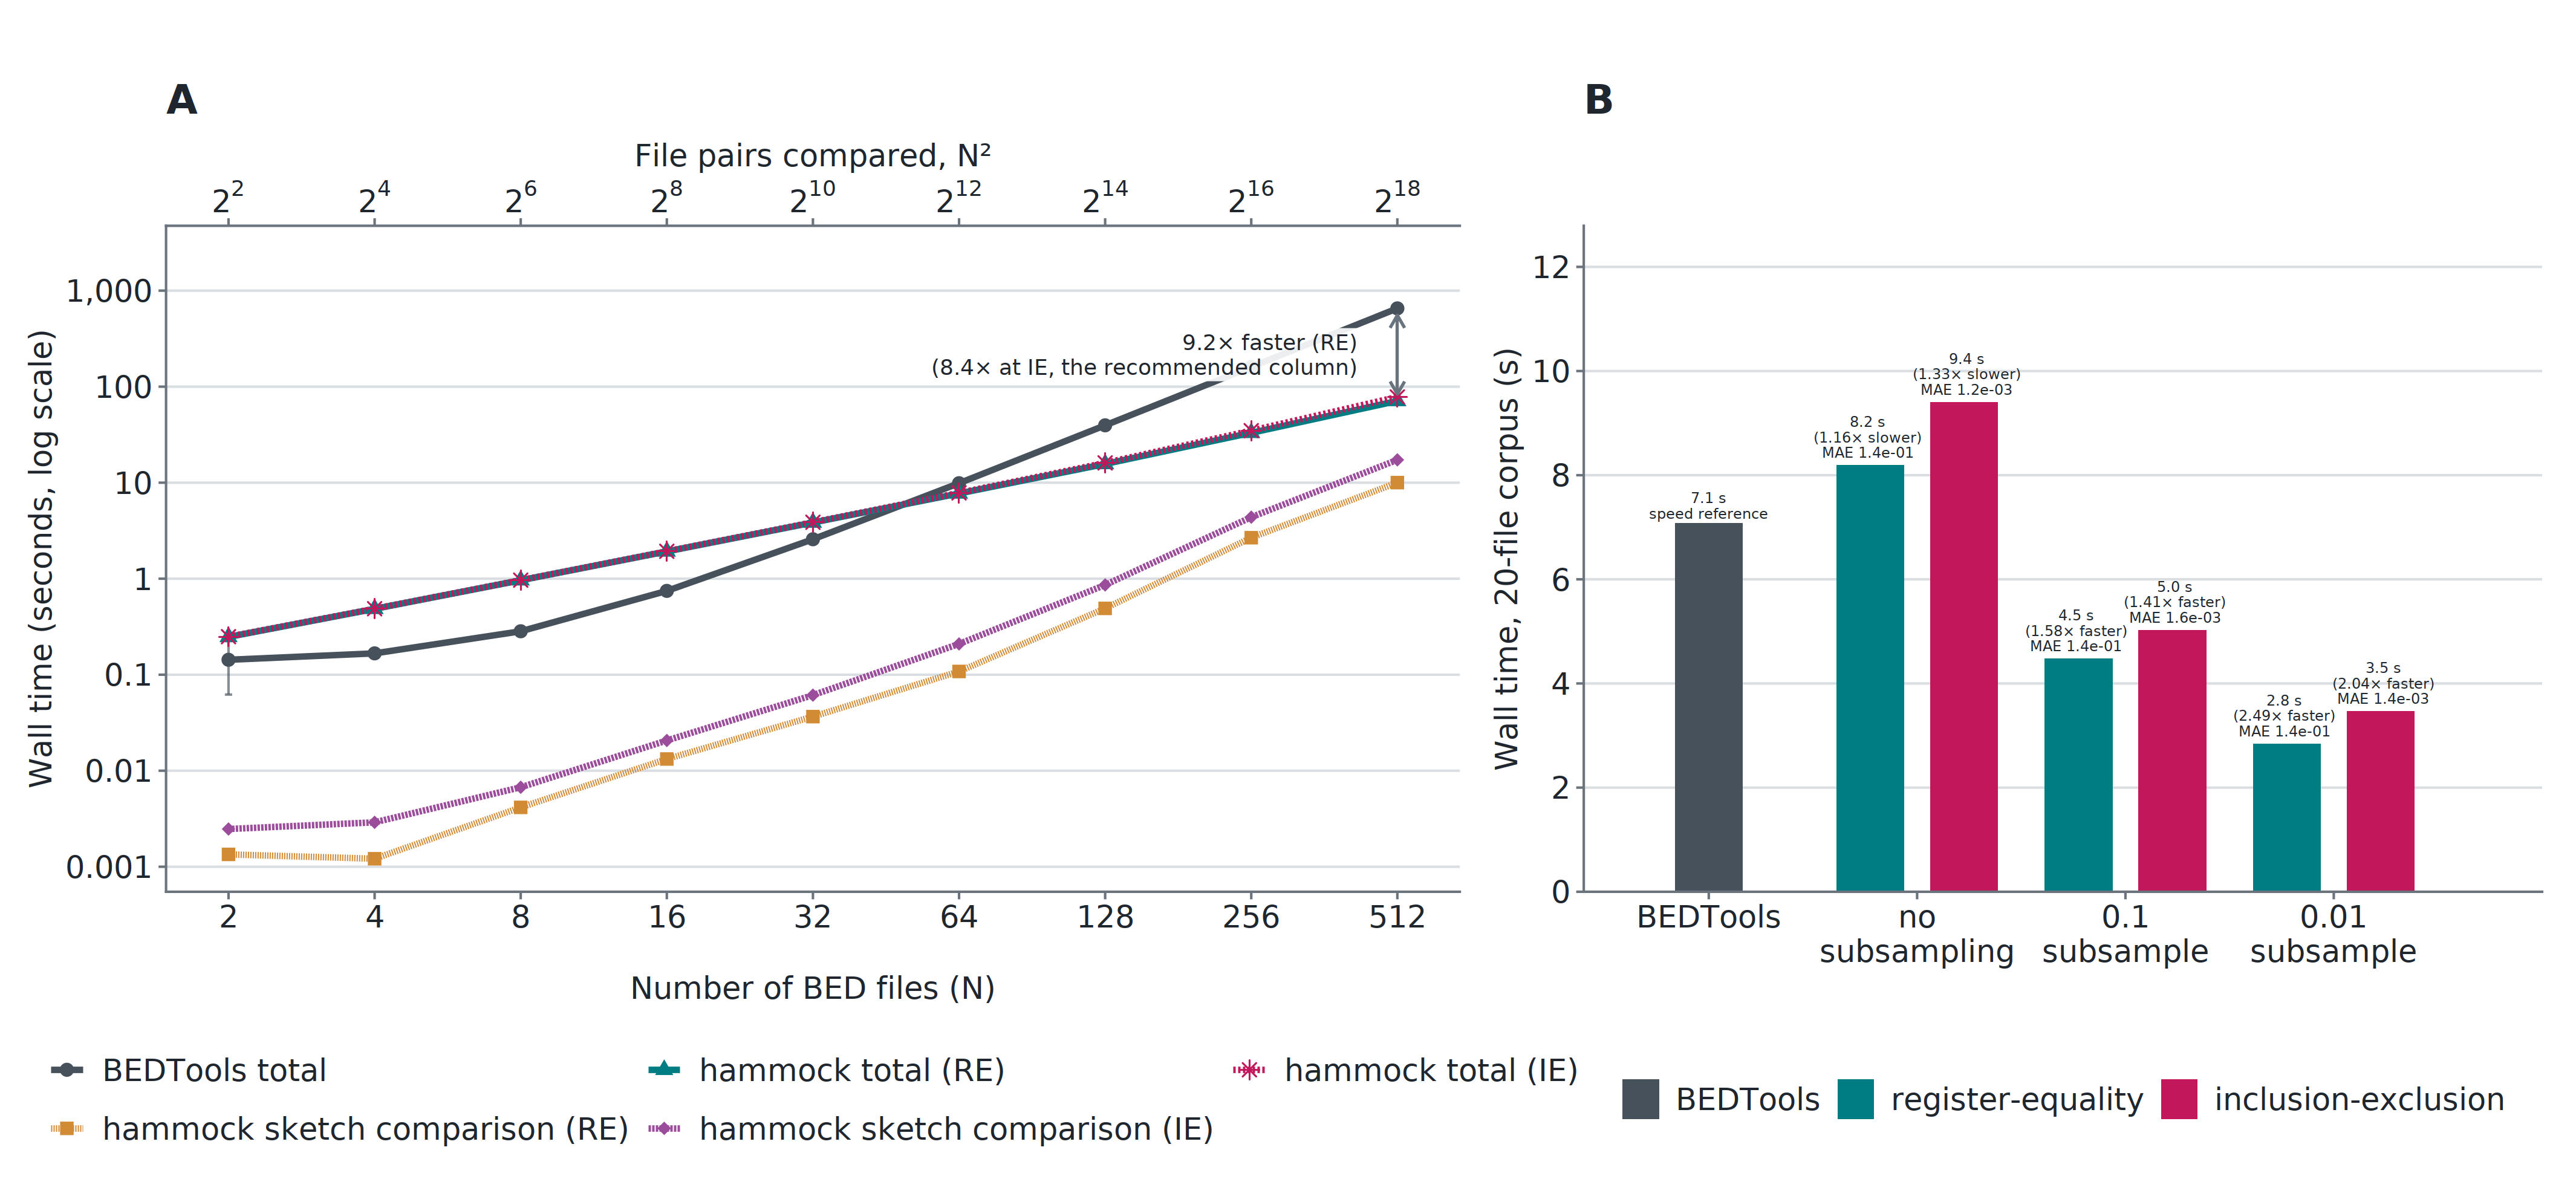
\includegraphics[width=\linewidth]{figures/pairwise_scaling_supplement.png}
    \caption{\textbf{Register-equality and inclusion--exclusion similarity differ in accuracy and computational cost.} (A) \textbf{Sketch reuse increases the advantage as collections grow.} Wall time across synthetic collections containing 10,000 intervals per BED file, using HyperLogLog precision $p=18$, 16 threads, and a full cross-product comparison of two $N$-file collections. Curves show BEDTools total wall time and, for both register equality (RE) and inclusion--exclusion (IE), hammock total wall time and the sketch-comparison component. At $N=512$, hammock was $9.2\times$ faster than BEDTools using RE and $8.4\times$ faster using IE. (B) \textbf{Subsampling further reduces runtime.} Wall time on the 20-file Maurano et al. fetal-tissue DNase hypersensitivity subset using interval mode with $p=18$ and eight threads. Bars compare BEDTools with hammock using RE or IE at \texttt{subB}=1.0, 0.1, and 0.01. Labels report wall time, speed relative to BEDTools, and mean absolute error relative to exact BEDTools Jaccard. Register-equality error remains approximately 0.14 across subsampling levels, whereas inclusion--exclusion error remains between 0.0012 and 0.0016.}
    \label{fig:pairwise_scaling_supplement}
\end{figure}

\subsection{Sequence-mode results using \texttt{jaccard\_similarity\_ie}}

\begin{figure}[htbp]
    \centering
    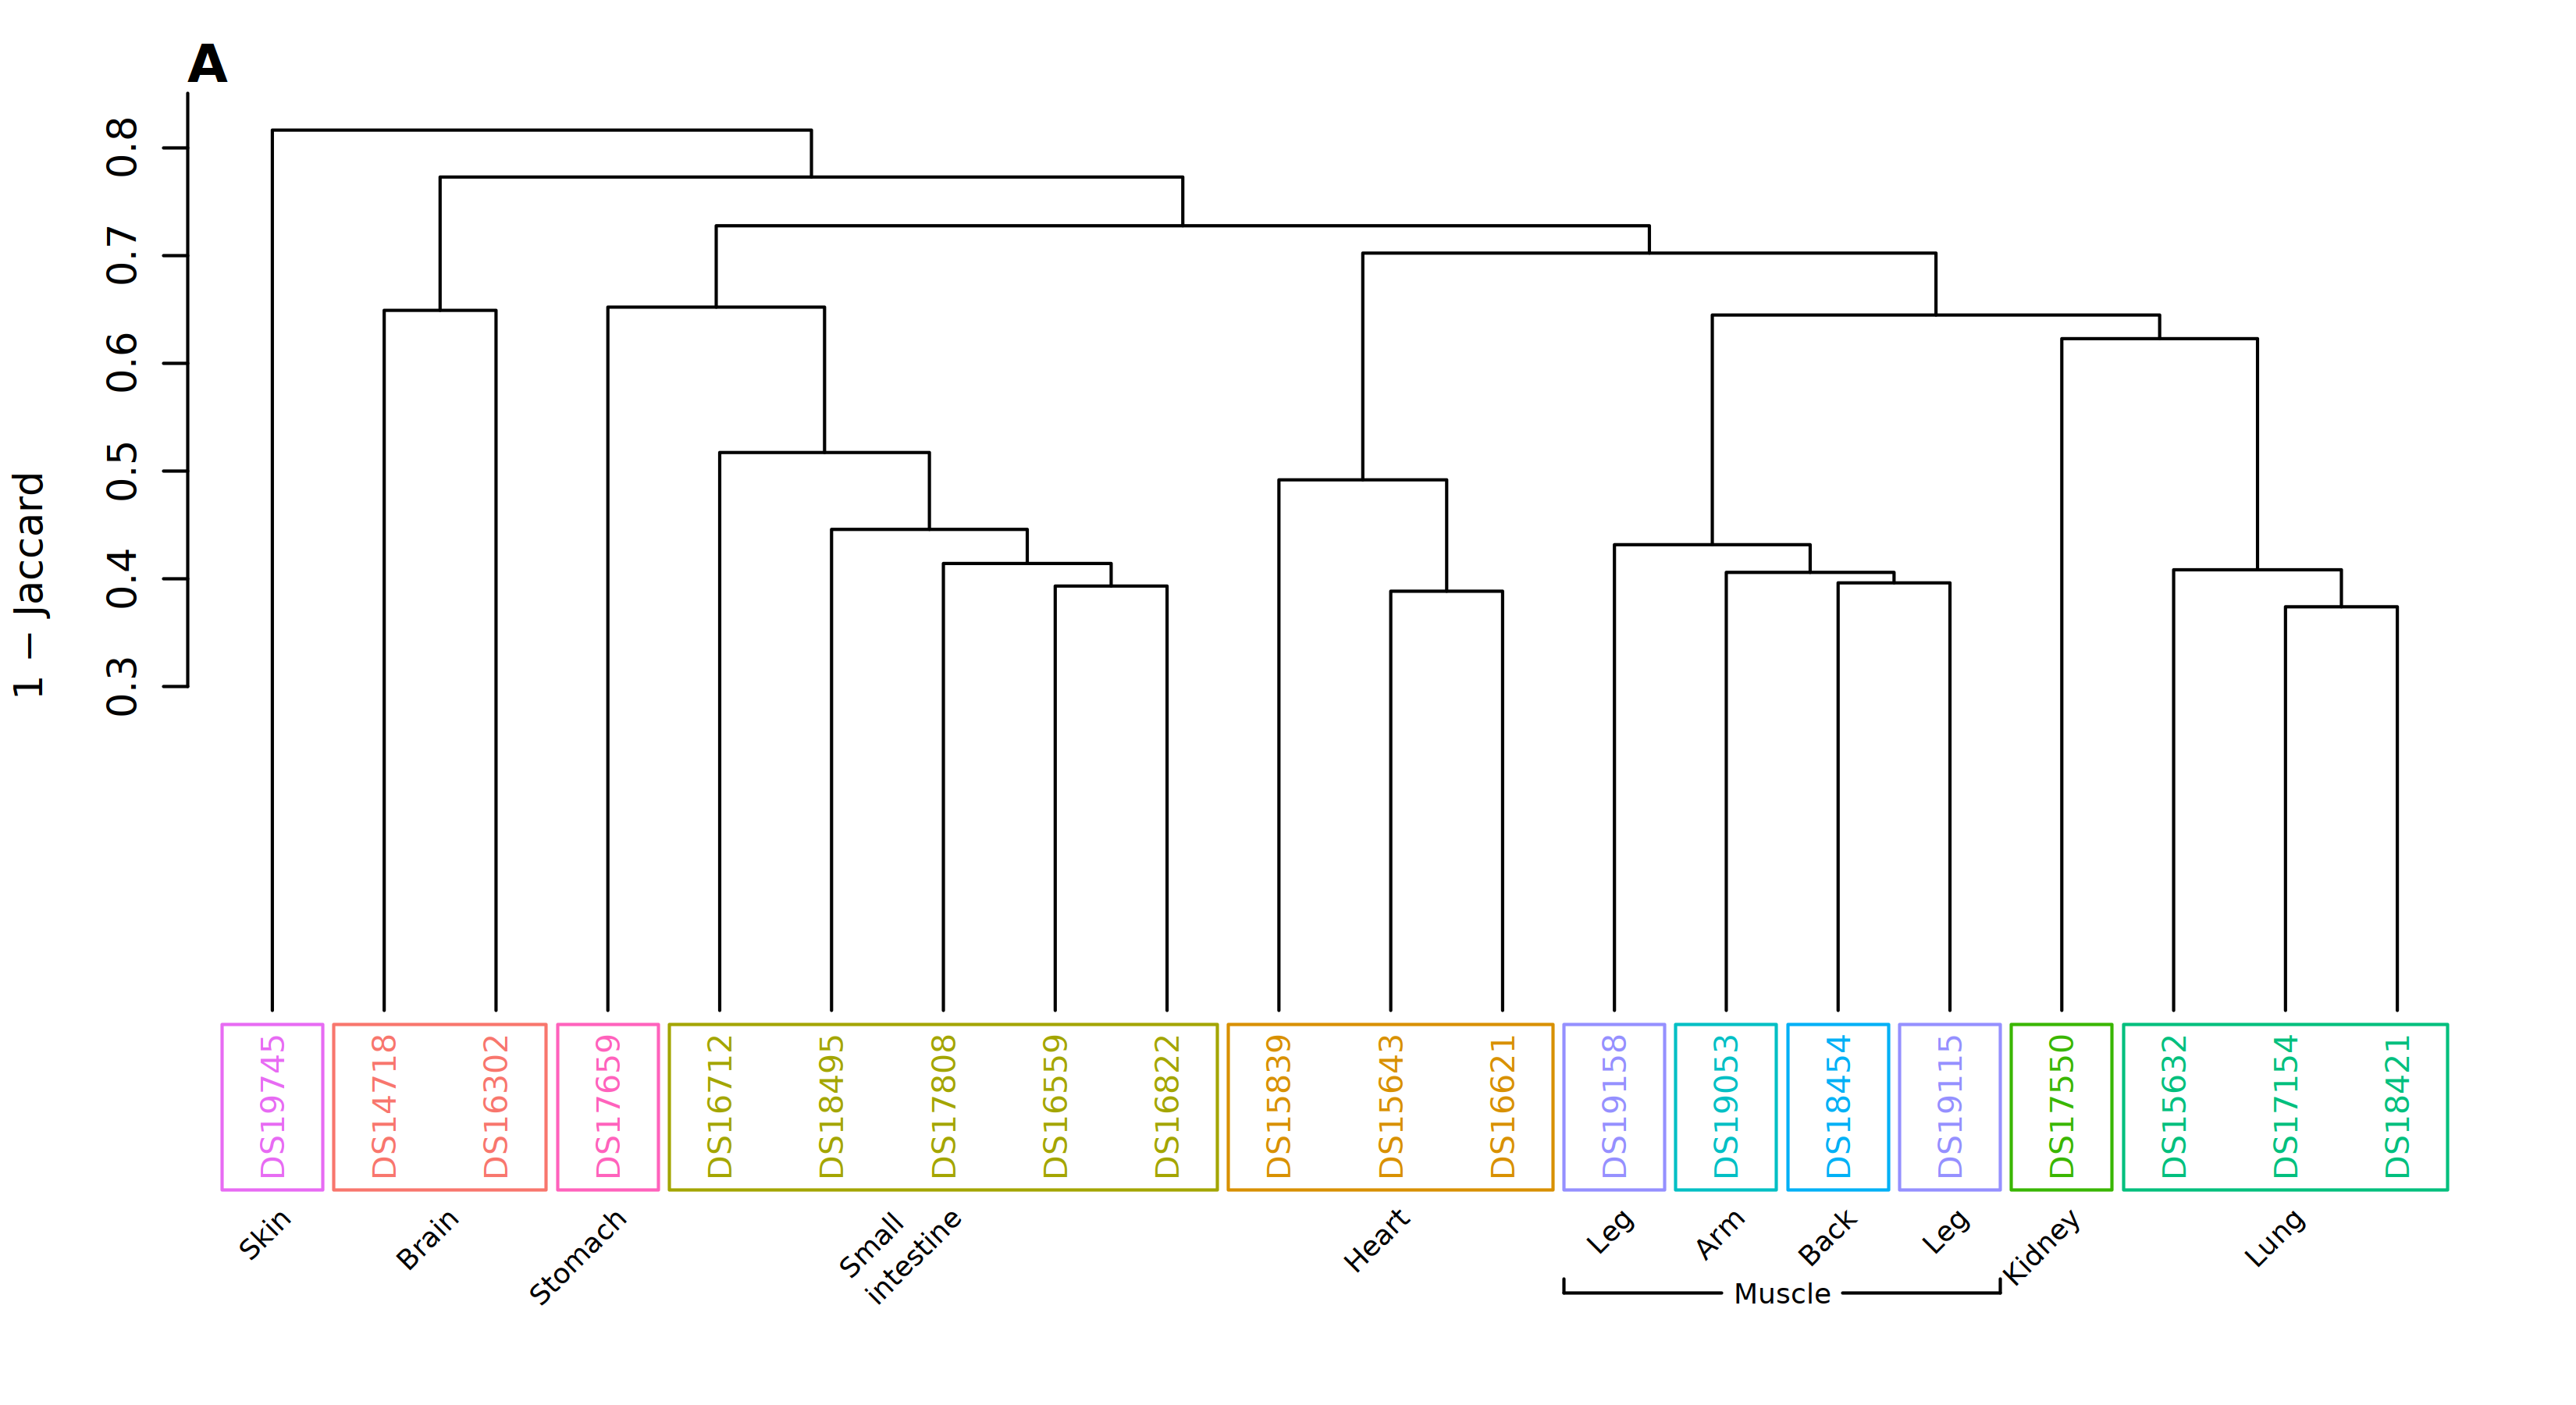
\includegraphics[width=\linewidth]{figures/sequence_tissue_clustering_k20_w20.png}
    \caption{\textbf{Numerical agreement with exact interval Jaccard does not maximize recovery of fetal-tissue organization.} (A) The same 20 fetal-tissue DNase-seq interval sets shown in main-text Figure~\ref{fig:sequence_tissue_clustering} were compared using the inclusion--exclusion Jaccard estimate, \texttt{jaccard\_similarity\_ie}, at $k=20$, $w=20$, and HyperLogLog precision $p=24$---the parameter combination with the greatest Pearson correlation with exact BEDTools Jaccard within the $p=24$ comparison shown in the main text ($r=0.99997$). Average-linkage agglomerative hierarchical clustering was performed on $1-J$. Leaf labels show dataset accessions and are colored and boxed by annotated tissue; these annotations do not represent a discrete cluster cut.}
    \label{fig:sequence_tissue_numerical_optimum}
\end{figure}

\begin{figure}[htbp]
    \ContinuedFloat
    \centering
    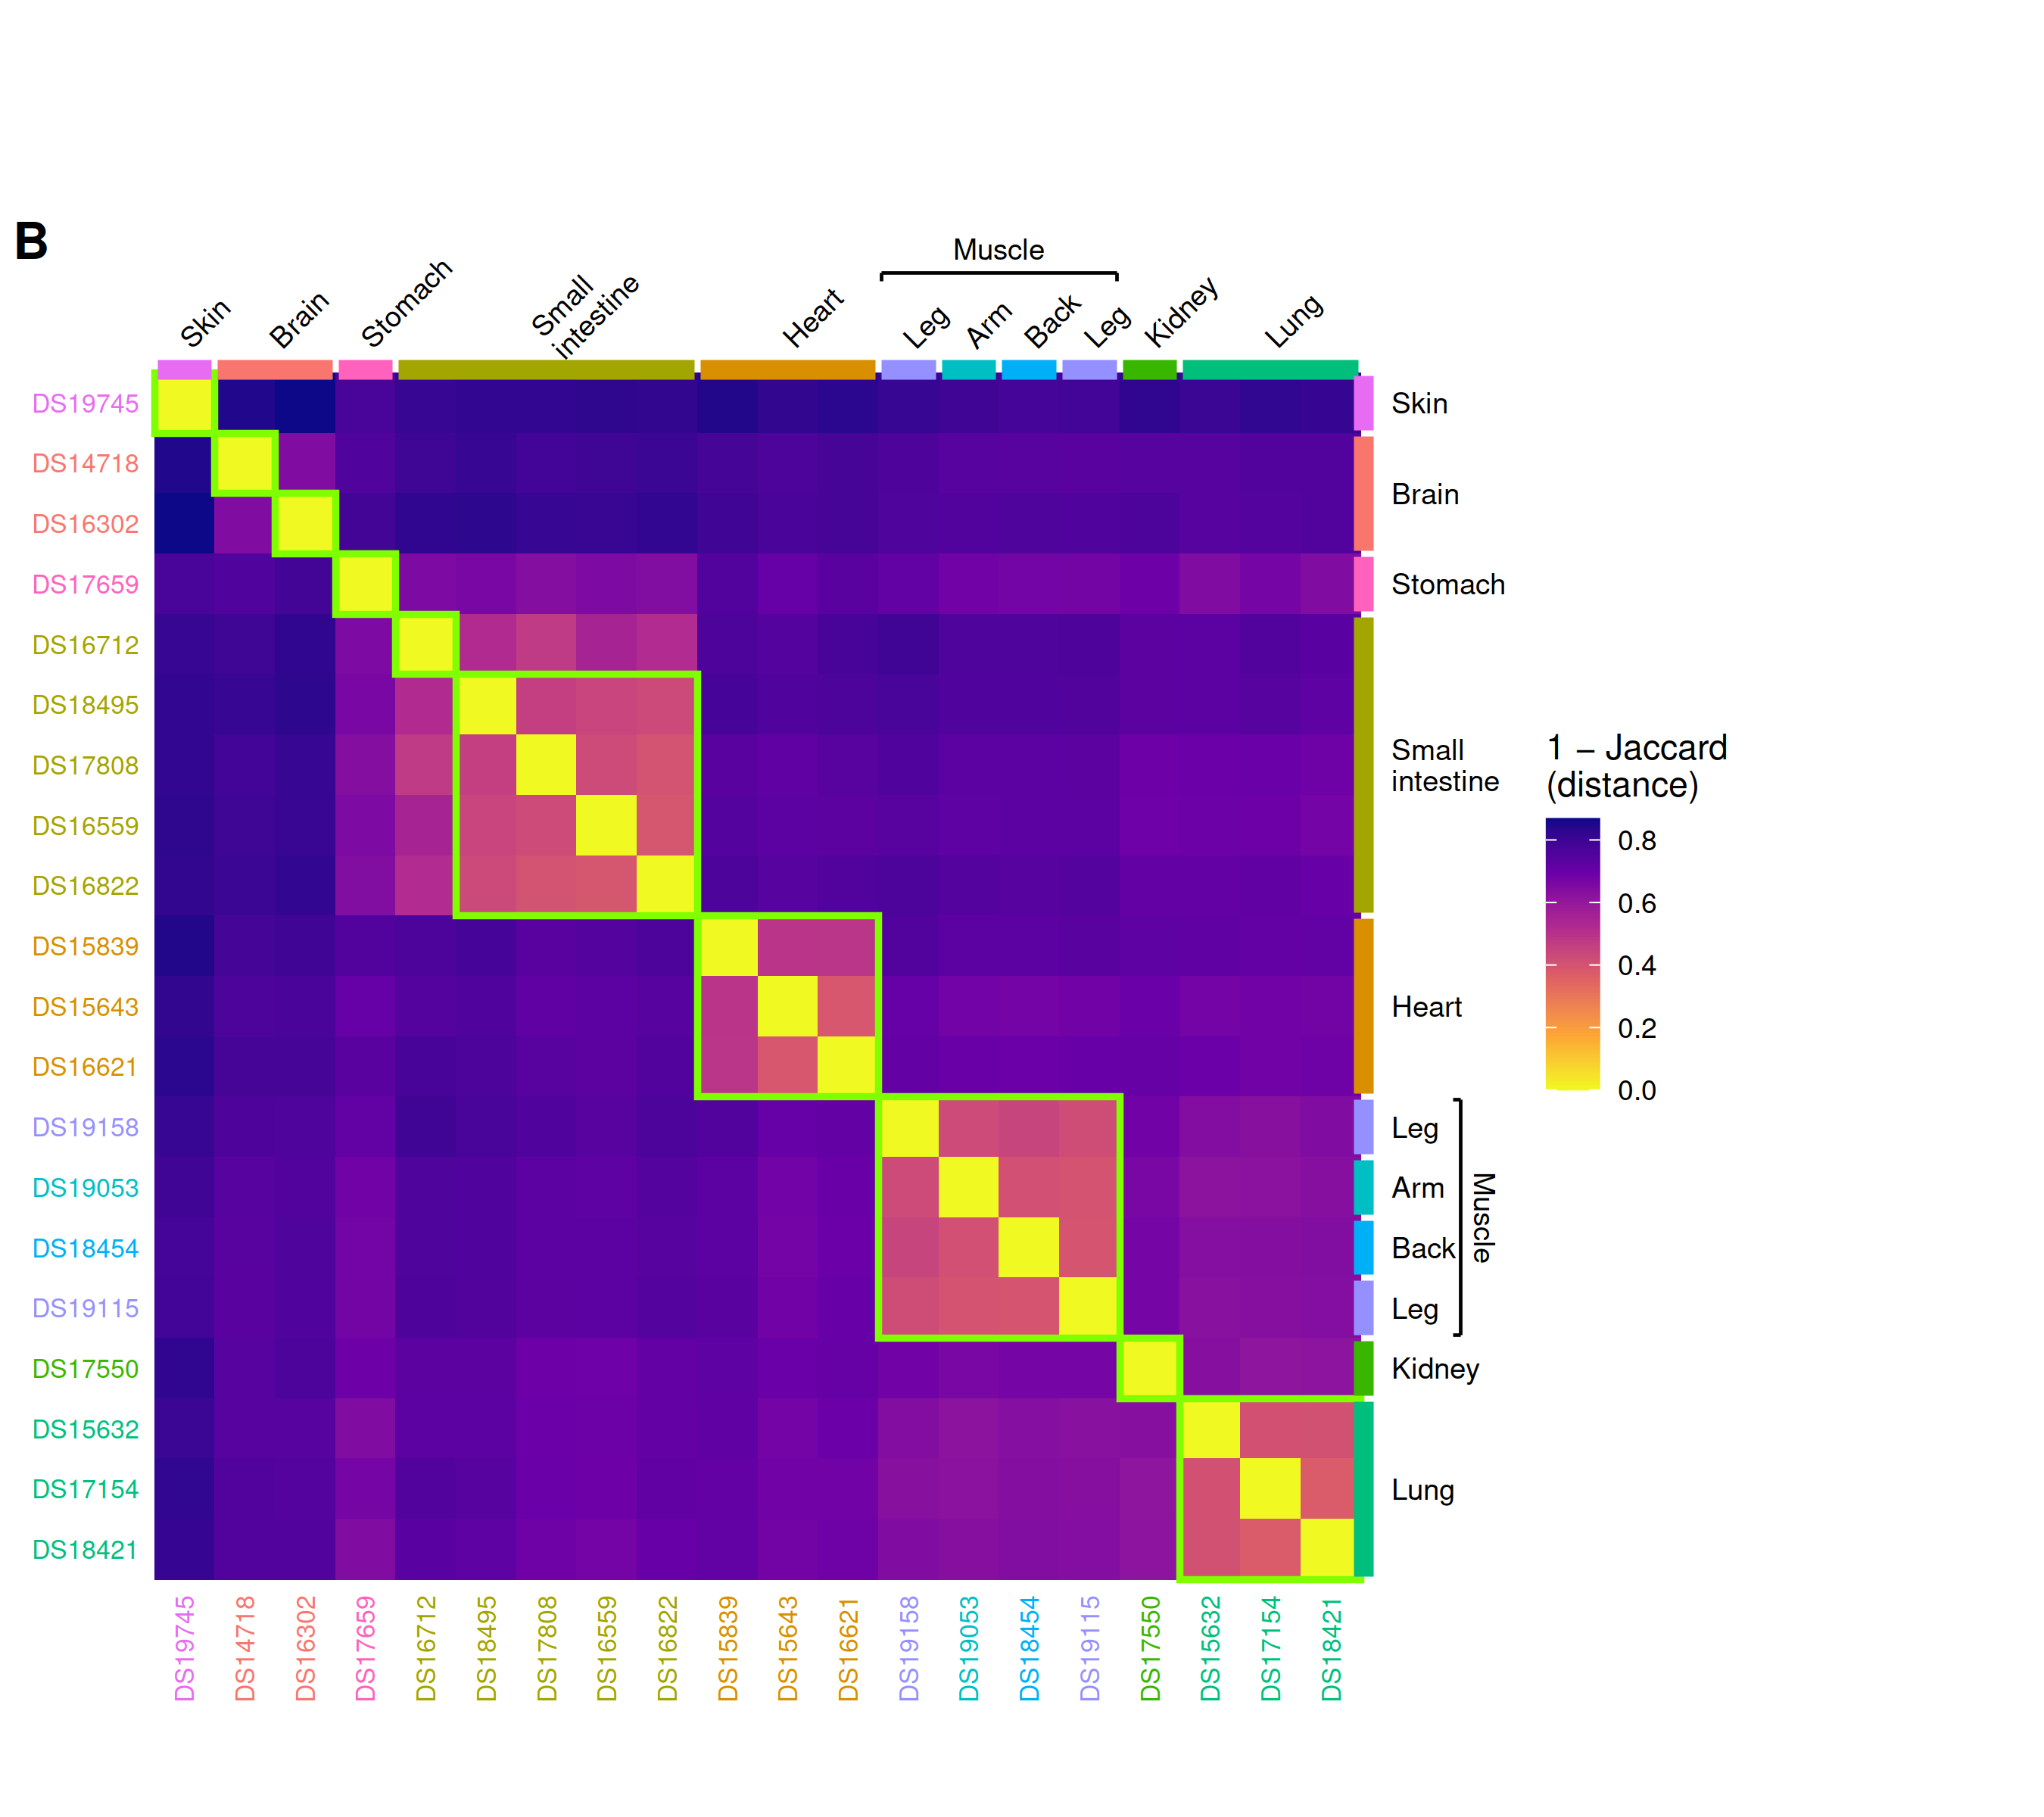
\includegraphics[width=0.68\linewidth]{figures/sequence_tissue_distance_heatmap_k20_w20.png}
    \caption[]{\textbf{Numerical agreement with exact interval Jaccard does not maximize recovery of fetal-tissue organization (continued).} (B) The complete pairwise $1-J$ distance matrix follows the dendrogram leaf order in A; this display ordering does not affect distances or cluster assignments. Accession-label colors and marginal bars denote the annotated tissues, with arm, back, and leg grouped under muscle. Lime-green diagonal outlines show the result of cutting the average-linkage agglomerative hierarchy into ten clusters. Relative to the annotated tissue partition, the cut separates the two brain samples, separates one of the five small-intestine samples, and combines the arm, back, and two leg samples into one cluster, yielding ARI $=0.693$ and NMI $=0.905$. In contrast, the biologically selected $k=10$, $w=30$ setting in main-text Figure~\ref{fig:sequence_tissue_clustering}, shown at the default $p=18$, yields ARI $=0.910$ and NMI $=0.961$. Thus, numerical agreement with exact pairwise Jaccard and recovery of tissue organization select different sequence-sketch parameters.}
\end{figure}

\subsection{Thread scaling}

\begin{figure}[htbp]
    \centering
    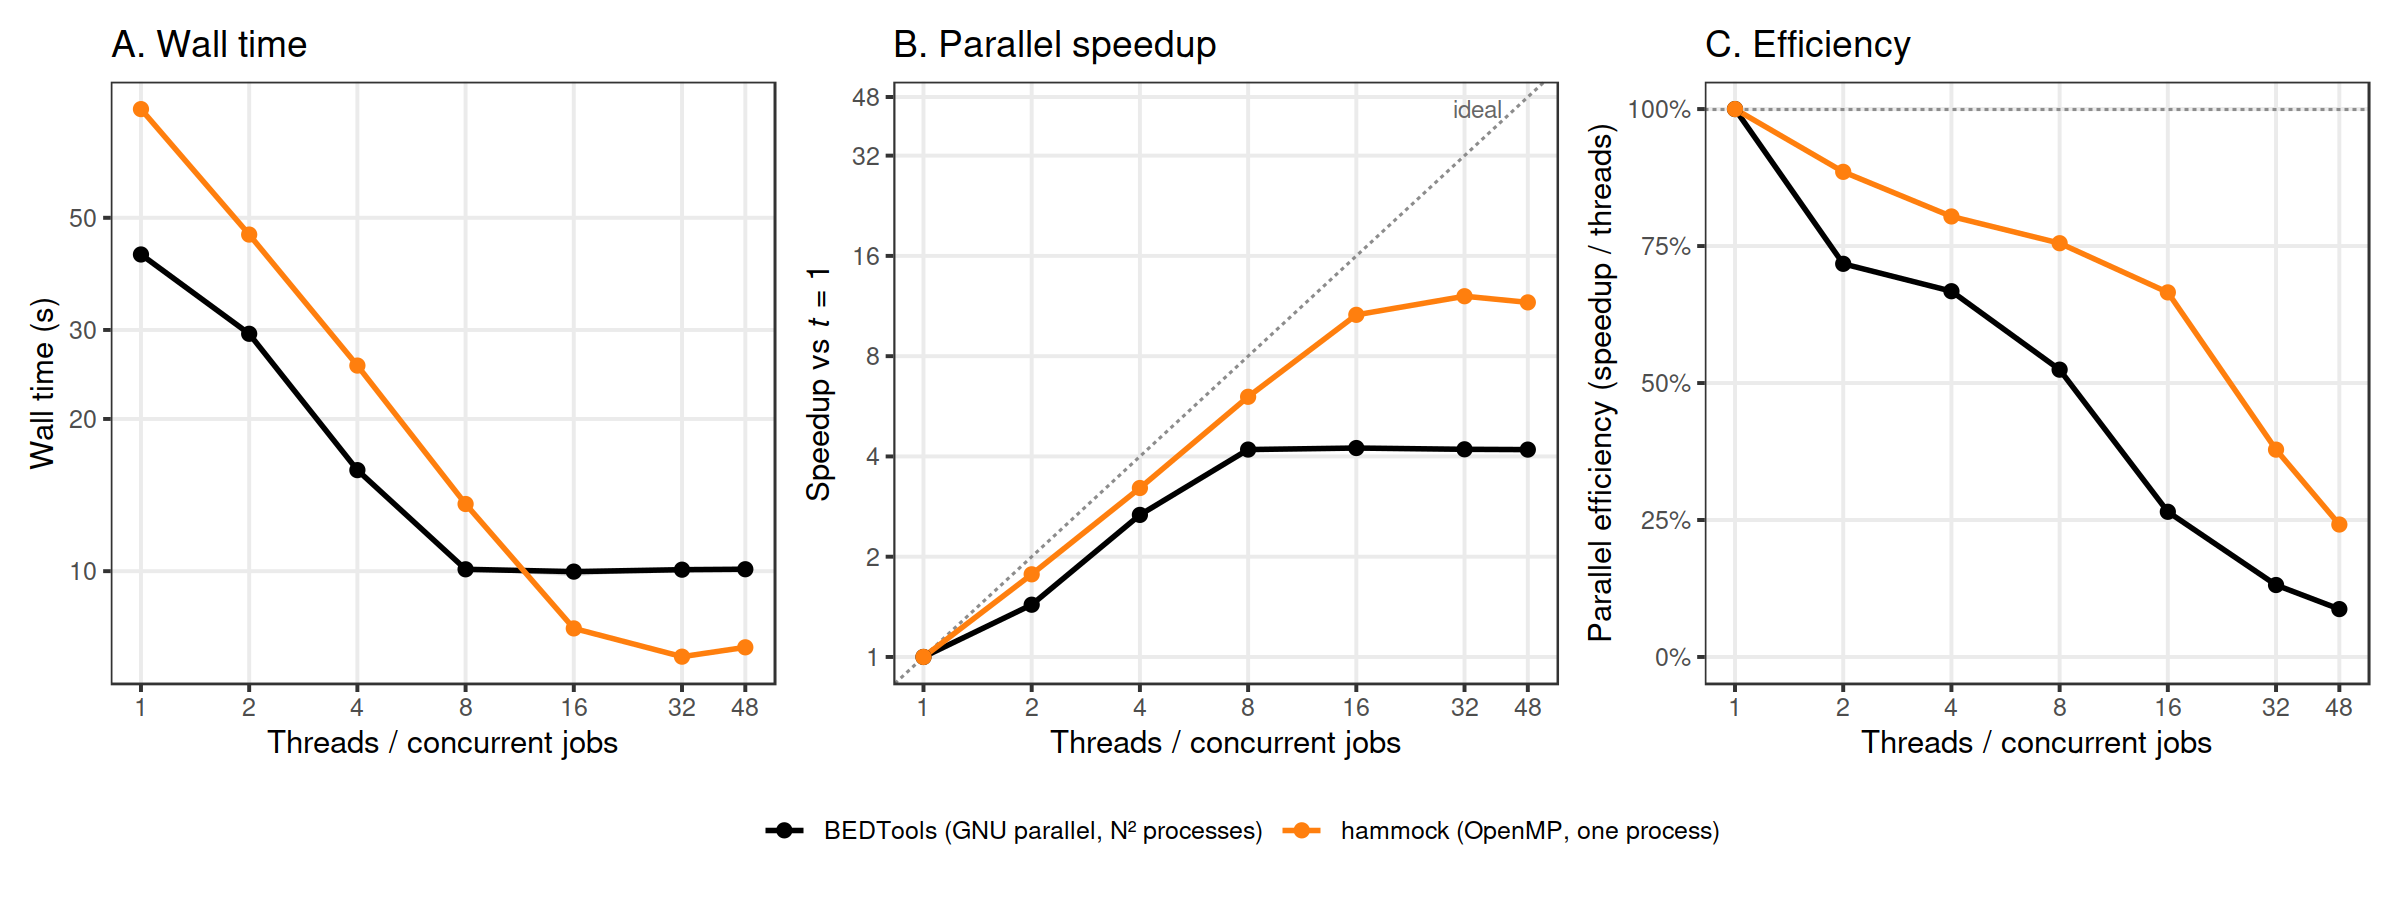
\includegraphics[width=\linewidth]{figures/threading_supplement.png}
    \caption{\textbf{The evaluated BEDTools all-pairs workflow saturates under process-level parallelization, whereas \program{hammock} continues to convert additional cores into throughput.} Wall time (A), speedup relative to each tool's own one-core execution (B), and parallel efficiency, defined as speedup divided by the allocated core count (C), were measured across allocations of 1--48 cores using two synthetic collections of 64 files each, with 10,000 intervals per file, HyperLogLog precision $p=18$, \texttt{subB}=1.0, and three replicates per configuration; curves summarize replicate medians. \program{hammock} used OpenMP threads within one process and the register-equality-only output mode; this benchmark did not measure the inclusion--exclusion output mode. Because \texttt{bedtools jaccard} is single-threaded and processes only one file pair per invocation, the BEDTools all-pairs workflow used GNU Parallel to run independent pairwise processes concurrently; the figure therefore evaluates workflow-level concurrency, not internal threading of a BEDTools process. BEDTools reached $4.22\times$ speedup at eight concurrent processes and remained nearly flat through 48 processes ($4.20\times$), while \program{hammock} reached $12.11\times$ speedup at 32 threads before declining slightly to $11.59\times$ at 48 threads. The absolute saturation level is system- and workload-dependent; the observed early plateau characterizes the evaluated process-per-pair workflow.}
    \label{fig:thread_scaling}
\end{figure}

\subsection{Catalog-scale performance}

\subsection{Sequence-mode parameter response}



\end{document}
